\section{Completion-preserving execution on discrete, delayed venues}
\label{sec:productionexecution}

The preceding impact and execution certificates do not by themselves
specify an order gateway. This section completes the interface between a
parent mandate, discrete child decisions, delayed private reports and a
finite decision model. The required ingredients are a pathwise commitment
ledger, a viability test and an explicit separation between optimization
and message delivery. Their guarantees concern the declared event maps;
exchange conformance remains a separate validation task.

\subsection{Normalized reports and a conserved parent ledger}

Consider a buy parent of $Q$ integer shares. Let $F$ be cumulative confirmed
fills, $r=Q-F$, and $o_i$ the upper bound on additional executable shares of
child $i$, including sent but unresolved messages.

\begin{remark}[Delayed cancellation and replacement]\label{prop:productionledger}
In the notation of this section, with $F$ cumulative confirmed fills and $o_i$
the reservation of child $i$, the invariant of Proposition~\ref{prop:reserve}
reads
\begin{equation}\label{eq:productionreservation}
  0\le F\le Q,\qquad o_i\ge0,\qquad \sum_i o_i\le Q-F.
\end{equation}
That proposition already covers messages in flight. Two of its clauses carry
the weight at a gateway. First, sending a cancel changes no reservation; only
an authoritative terminal report, after its cumulative executions are
reconciled, releases the remainder. Second, a replacement that can coexist with
the old order is two possibly executable children and must reserve both
quantities until the old order is resolved. A smaller joint reservation is
admissible only when the venue's replacement is atomic and its treatment of
in-flight fills is established.
\end{remark}

The normalized report contract is part of the proof. A terminal report may
arrive through a different channel from execution messages; receipt of a
public delete alone does not establish that all private fills were booked.
The adapter needs sequence recovery and reconciliation, including duplicate
reports and session-scoped identifiers. A trade correction is a new ledger
event, not a duplicate. During an unresolved gap, keep conservative exposure
and prevent new commitments that rely on the missing information. The
reference code verifies this normalized contract; it does not implement the
entire Nasdaq OUCH or NYSE Pillar protocol \citep{ouch}.

For $Q=10$, a child reserving six shares leaves room for only four more.
If a cancel request incorrectly releases those six shares, a replacement
of ten can coexist with the original six and expose the parent to sixteen.
Correctly retaining the reservation prevents this overcommitment before
any distributional assumptions about fills are used.

\subsection{Feasibility is stronger than an expected fill forecast}

Let $\mathcal S_k(x,a)$ be the union of possible successor states over the
admitted event laws, including delayed-message outcomes. The state contains
both $r$ and all $o_i$. Define a terminal set
$\mathcal V_N=\{x:r(x)=0,\ \sum_i o_i(x)=0\}$ and recursively
\begin{equation}\label{eq:viabilityrecursion}
 \mathcal V_k=\left\{x:\exists a\in A_k(x),\quad
                 \mathcal S_k(x,a)\subseteq\mathcal V_{k+1}\right\}.
\end{equation}

\begin{theorem}[Robust completion by an admissibility mask]
\label{thm:productionviability}
In a finite-horizon finite-state model with nonempty outcome supports,
$x\in\mathcal V_k$ if and only if there is a policy that reaches
$\mathcal V_N$ for every allowed sequence of outcomes from $x$.
Choosing only actions whose successors lie in $\mathcal V_{k+1}$ preserves
this guarantee under arbitrary reoptimization within that mask.
\end{theorem}
\begin{proof}
At $N$ the assertion is the definition. If an action has every successor
in $\mathcal V_{k+1}$, the induction hypothesis supplies a completing
continuation after each successor. Conversely, a policy completing under
every outcome must choose a first action all of whose successors admit a
completing continuation, hence satisfy \eqref{eq:viabilityrecursion}.
The argument applies after each realized transition and proves the
reoptimization statement.
\end{proof}

This is the finite-horizon target-tube recursion of
\citet{BertsekasRhodes1971}; \citet{Aubin1991} develops the general viability
theory. Its use here is the explicit inclusion of unresolved messages in the
successor supports.

This is a worst-case support guarantee, stronger than high expected fills.
It can be empty if a halt, failed connectivity or unavailable liquidity
makes completion impossible. The optimizer must then report infeasibility
or a separately authorized mandate relaxation; it cannot manufacture
liquidity through a terminal penalty.

A useful terminal specialization has no unresolved orders after the current
stage, a remaining requirement $r$, and a guaranteed next-stage immediate
capacity $C$. If the current action produces fills
$f\in[f_{\min},f_{\max}]$, with integer bounds and $0\le f_{\max}\le r$,
completion for every outcome is possible exactly when
\begin{equation}\label{eq:capacityworstfill}
 r-f_{\min}\le C.
\end{equation}
Necessity follows from the worst fill; sufficiency follows by purchasing
$r-f$ at the next stage. With $r=5$, $C=3$, an action guaranteeing at least
two fills is feasible. A passive order with mean fill four but a possible
zero fill is infeasible for this guarantee. When live children remain,
\eqref{eq:capacityworstfill} alone is insufficient: cancellation resolution
and joint outstanding exposure belong in the full viability recursion.

\subsection{Integer allocation rather than independent rounding}

Ticks constrain prices, and share or lot grids constrain quantities. The
continuous allocation problem is a benchmark; its components cannot be
rounded independently without checking total quantity and capacity.
Consider $m$ destinations, integer capacities $C_i$, integer parent $Q$,
and separable costs $c_i(n)$ for $n=0,\ldots,C_i$, with $c_i(0)=0$.
Assume discrete convexity: the marginal costs
$d_i(n)=c_i(n)-c_i(n-1)$ are nondecreasing in $n$.

\begin{classical}[Exact integer marginal allocation]
\label{prop:integerallocation}
If $Q\le\sum_i C_i$, repeatedly assigning the next unit to a destination
with the smallest available next marginal cost gives a feasible minimizer
of $\sum_i c_i(n_i)$ subject to $\sum_i n_i=Q$ and $0\le n_i\le C_i$.
Ties can be resolved by any fixed deterministic rule.
\end{classical}
\begin{proof}
Every feasible allocation selects $Q$ marginal costs and, for each
destination, a prefix of its nondecreasing sequence. The greedy selection
always takes a smallest unselected available marginal. Any unavailable
later marginal is at least its available predecessor, so no cheaper
unselected marginal is missed. Thus it selects $Q$ globally smallest
marginals in a prefix-feasible order. No other sum of $Q$ marginals is lower.
\end{proof}

Greedy marginal allocation for separable discrete-convex costs is classical
\citep{Gross1956,IbarakiKatoh1988}; it is recorded here because the separable convex routing cells of Section~\ref{sec:routing} satisfy
its hypotheses once lot and capacity grids are fixed.

For $c_1(n)=n^2/2$, $c_2(n)=n^2$, $Q=5$ and capacities at least five,
the continuous optimum is $(10/3,5/3)$ with cost $25/3$. The integer
optimum is $(3,2)$ with cost $17/2$ and an integrality gap $1/6$.
This example concerns guaranteed quantities with separable costs. Random
fills, coupled impact or shared fee tiers generally destroy separability;
then the finite joint action set must be optimized directly. Likewise,
rounding a price can change queue rank and fill law discontinuously, so a
smooth rounding-error estimate is not automatic.

\subsection{Joint scenarios and a runnable reference controller}

At each decision, use outcomes of the form
\[
 (\hbox{fills},\hbox{execution prices},\hbox{fees},
   \hbox{elapsed time},\hbox{reports},\hbox{next book state}).
\]
The planner first applies the reservation and viability masks, then compares
negative implementation shortfall plus continuation reward. Report each
cost component in cash or a clearly stated per-parent normalization;
a fill-conditioned spread is not the same unit as full-parent shortfall.
A marketable limit can control price while failing to complete; a completion
assumption must therefore include the available liquidity and allowable
prices, not just an order label.

The package includes a deterministic discrete-event engine with separate
exchange-event and local-receipt times, a tagged FIFO queue cell and a
normalized commitment ledger. The FIFO cell is a declared mathematical
mechanism. It is not a representation of NYSE's participant parity rules
\citep{nysefaq}. The simulator retains fills between a cancel request
and its effective exchange cancellation. Receipt-time callbacks cannot
read future exchange events. The example records both clocks and tests a
fill that precedes effective cancellation even though the cancel was sent
first. Transport gap recovery and exchange-specific binary decoding remain
adapter obligations, not implied capabilities of the reference engine.

A production loop has four ordered operations: reconcile available reports;
construct an admissible joint action; reserve and send its actual child
messages; then evaluate the emitted action and its outcomes. The calibration
and implementation theorem in Section~\ref{sec:deploymentcalibration}
compares this emitted policy to the optimum in the same feasible model.
Hardware timeouts and stale observations must be represented in its state
or error allowances. They are not free perturbations of a schedule.

\subsection{Synthetic end-to-end checks and interpretation}

\begin{table}[htbp]
\centering\small
\caption{Execution implementation checks. Share counts and costs are
synthetic; the latency trace uses arbitrary clock units.}
\begin{tabular}{p{.55\linewidth}r}
\toprule
Quantity & Value\\\midrule
\inputtable{tables/production_rows.tex}
\bottomrule
\end{tabular}
\end{table}

The new suite exhaustively compares greedy integer allocation with all
feasible small allocations, checks the worst-fill capacity condition,
and exercises partial fills, duplicate normalized reports, rejection,
non-atomic replacement, cancel races and conservative recovery states.
Random finite decision models independently check the policy-transfer
bound by exact backward evaluation. These checks support the stated
algorithms and identities. 


\begin{figure}[htbp]
\centering
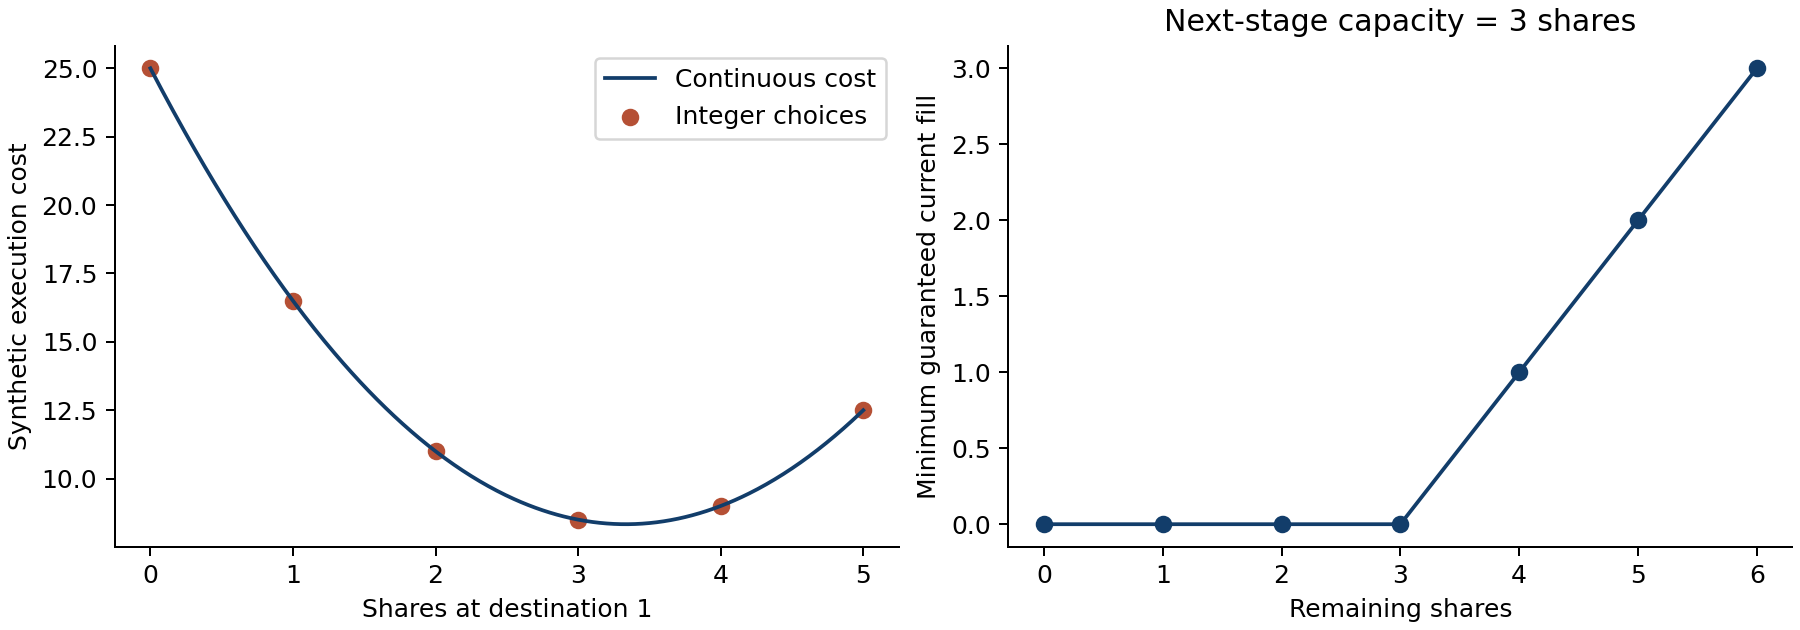
\includegraphics[width=\linewidth]{figures/07_production_bridge.png}
\caption{Discrete implementation diagnostics generated by the accompanying
reference suite. All axes use synthetic model units; the curves illustrate
the declared mechanisms rather than estimated market behavior.}
\label{fig:productionbridge}
\end{figure}

\subsection{Persistent flow and endogenous conditioning}
Under a fixed stationary Markov policy, a finite irreducible
continuous-time book chain is exponentially mixing. Bounded state observables
then have exponentially decaying stationary covariances. This does not follow
for arbitrary adaptive controls from the controlled-book assumptions alone.
\citet{RodriguezDominguez2026Switching} derives long-memory flow from switching frictions
and heterogeneous horizons. A finite-state approximation to that asymptotic persistence requires
an explicit truncation or model-error allowance, charged via
the primitive budget of Theorem~\ref{thm:bookcoupling} or the reference defect
of Proposition~29.13; a finite state fitted to autocorrelations alone carries no
such charge. \citet{RodriguezDominguez2026Market} makes the conditioning
representation itself an equilibrium object. For the present results this bears
on one hypothesis: the reference law in Proposition~29.13 and the uncertainty
family in Section~\ref{sec:baselineexecution} are fixed, whereas widespread adoption of a common
representation can move the law those bounds must contain.

